% AXIOM @ NeurIPS 2026 -- 4 pages excluding references and appendix.
% Double-blind: keep the anonymous option until acceptance.
%
% Needs neurips_2026.sty (from the NeurIPS 2026 template bundle) alongside this file.
% Falls back to plain article so the skeleton compiles for local preview without it.
\documentclass{article}
\IfFileExists{neurips_2026.sty}{\usepackage[dblblindworkshop]{neurips_2026}}{%
  \usepackage[margin=1in]{geometry}\usepackage{natbib}
  \providecommand{\workshoptitle}[1]{}}
\workshoptitle{AXIOM: Predictive Principles for Efficient AI}

\usepackage[utf8]{inputenc}
\usepackage[T1]{fontenc}
\usepackage{hyperref}
\usepackage{url}
\usepackage{booktabs}
\usepackage{amsfonts}
\usepackage{amsmath}
\usepackage{amsthm}
\usepackage{nicefrac}
\usepackage{microtype}
\usepackage{graphicx}

\newtheorem{proposition}{Proposition}
\newtheorem{corollary}{Corollary}
\newtheorem{lemma}{Lemma}

\title{What Does a Network Know at Initialisation?\\
Measuring the Dynamics of Parameter-Wise Functional Sensitivity}

\author{Anonymous}

\begin{document}
\maketitle

\begin{abstract}
Parameter-wise functional sensitivity, $S_i(\theta)=\mathbb E_x\|\partial F_\theta(x)/\partial\theta_i\|_2^2$,
measures how strongly the realised function responds to perturbing one parameter. It is
label-free and loss-free, and is exactly the diagonal of the parameter-space Gram matrix
dual to the empirical NTK. Pruning methods increasingly rely on the \emph{ordering} such
scores induce, often computed early in training or at initialisation. We ask when that
ordering settles, and find that answering the question requires fixing how it is measured.
Sensitivity spans orders of magnitude across layers, so a global top-$k$ set largely encodes
a per-layer budget: on a control whose two rankings share \emph{nothing} within any layer,
raw top-$k$ overlap is $0.83$ and Spearman $\rho$ is $0.98$, while chance-corrected agreement
is $-0.004$. Measuring against a layer-budget-matched baseline, and against a ceiling set by
resampling the estimation data, we find (i) the ordering does not freeze: it reorganises
throughout training, in converged models, at constant learning rate, for every architecture
we tested; (ii) at initialisation it carries essentially no within-layer information about
the final ordering --- all apparent agreement is the layer budget; and (iii) what \emph{is}
predictable is how stable the top-$k$ boundary is, from the tail index of the sensitivity
spectrum. We give a bound explaining (iii): rank churn is controlled by Jacobian motion,
which vanishes in the linearised regime, and boundary crossings are limited by the local
density of a heavy-tailed spectrum. % TODO(final): headline numbers once E8 lands.
\end{abstract}

\section{Introduction}
%% TODO(final): 3 paragraphs.
%%  P1  over-parameterisation, pruning wants to act early, prune-at-init underdelivers.
%%  P2  the object we track is functional (label-free), not a loss saliency; the question
%%      is not "is this weight important" but "when does the ANSWER stop changing".
%%  P3  contributions, below.

\paragraph{Contributions.}
\begin{itemize}
\item A measurement protocol for rank stability robust to the two failure modes that make
      naive versions vacuous: estimator noise, handled by a ceiling from disjoint data
      folds, and layerwise scale separation, handled by chance correction against a
      layer-budget-matched baseline. We also report the \emph{pairwise} checkpoint
      agreement matrix, which distinguishes "the ordering froze" from "the ordering is
      still moving and $t$ is merely closer to $T$" --- a distinction the usual
      agreement-with-final curve cannot make, being pinned to $1$ at $t=T$. % Sec 3
\item The finding that the sensitivity ordering \emph{does not} freeze: it reorganises
      throughout training in converged models at constant learning rate, so reports of
      early stability appear to rest on uncorrected metrics. % Sec 4
\item The finding that at initialisation $S$ carries essentially no \emph{within-layer}
      information about the final ordering; all apparent agreement is the layer budget.
      This suggests sensitivity-based pruning at initialisation operates through layerwise
      allocation rather than within-layer selection. % Sec 4
\item A bound tying rank churn to Jacobian motion and to the local density of the
      sensitivity spectrum, predicting that boundary stability increases with tail
      heaviness --- confirmed across architectures, including the sign of the intermediate
      variable --- plus a causal test using an explicit laziness parameter. % Sec 5
\end{itemize}

\section{Parameter-wise functional sensitivity}
\label{sec:sensitivity}
%% Reused from the companion draft (Sec. 2), compressed to the essentials.
Let $F_\theta:\mathcal X\to\mathbb R^{d_y}$ and let $\mu_{\mathcal X}$ be the input
distribution. The parameter-wise functional sensitivity score is the squared
$L^2(\mu_{\mathcal X})$ norm of the Fr\'echet derivative of the parameter-to-function map,
taken coordinate-wise:
\begin{equation}
  S_i(\theta):=\mathbb E_{x\sim\mu_{\mathcal X}}
  \big[\|\partial F_\theta(x)/\partial\theta_i\|_2^2\big].
  \label{eq:S}
\end{equation}
With $G_\theta\in\mathbb R^{nd_y\times p}$ the empirical Jacobian feature matrix,
$Q_\theta=\frac1n G_\theta^\top G_\theta$ and $K_\theta=\frac1n G_\theta G_\theta^\top$ are
dual Gram matrices; $(Q_\theta)_{ii}=\widehat S_i(\theta)$ and
\begin{equation}
  \operatorname{tr}(K_\theta)=\operatorname{tr}(Q_\theta)=\sum_{i=1}^p\widehat S_i(\theta).
  \label{eq:trace}
\end{equation}
Functional sensitivity therefore decomposes the NTK trace into parameter-wise
contributions. Crucially \eqref{eq:S} refers to no loss and no label: it is a property of
the realised function, which is what allows the same quantity, and the same measurement
code, to be applied unchanged to a classifier and to a language model.

\paragraph{Estimation.}
We estimate \eqref{eq:S} with per-example gradients. For $d_y$ small we sum exactly over
output coordinates, giving an estimator with no probe noise; for large $d_y$ we use
Rademacher probes $r$ with $\mathbb E[rr^\top]=I/d_y$. We verify the two agree and that
$K_{jj}=\sum_i \widehat S_i(\theta;x_j)$, the per-example form of \eqref{eq:trace}.
% NOTE: squaring a batch-averaged gradient estimates (E g)^2, not E[g^2]; the two differ
% by the gradient covariance. Per-example is the definition in \eqref{eq:S}.

\section{Measuring the stability of an ordering}
\label{sec:protocol}
%% This section is a contribution, not boilerplate: it is what makes the headline claim
%% survive contact with the two standard objections.
A ranking claim needs a scale. We use the top-$k$ keep-set $A_k$ a pruner at sparsity
$1-k/p$ would select, and report overlap $|A_k(\theta_t)\cap A_k(\theta_T)|/k$.

\paragraph{Chance correction.}
Sensitivity varies by orders of magnitude \emph{across} layers, so a global top-$k$ set
largely encodes a per-layer budget and two unrelated rankings share most of it for free.
We report the chance-corrected quantity
\begin{equation}
  \mathrm{adj}=\frac{\mathrm{obs}-\mathrm{chance}}{1-\mathrm{chance}},\qquad
  \mathrm{chance}=\frac1k\sum_{\ell}\frac{k_\ell(\theta_t)\,k_\ell(\theta_T)}{p_\ell},
\end{equation}
the overlap expected if both sets kept their layer budgets but placed picks at random
within each layer. % TODO(final): cite the random-ticket sanity check here.
On a synthetic control whose two rankings share nothing within any layer, raw overlap is
$0.83$ and Spearman $\rho$ is $0.98$, while $\mathrm{adj}=-0.004$.

\paragraph{A measurement ceiling, and a threshold-free $t^*$.}
$\widehat S$ is estimated on finitely many inputs, so no agreement can exceed the
agreement of two independent estimates at the \emph{same} parameters. We split the
estimation set into disjoint folds, compare them at every checkpoint, and Spearman--Brown
correct to full sample size. This turns the headline into an operational statement with no
free threshold:
\begin{equation}
  t^*:=\min\{t:\ \text{further training moves the ordering less than resampling the data does}\}.
\end{equation}
This is the trajectory counterpart of the estimation-error bound for the conditional
population ranking: the two error sources are placed on one axis and we report the
crossing. % TODO(final): cross-reference the companion draft's Lemma.

\section{The ordering freezes early}
\label{sec:results}
\begin{figure}[t]\centering
  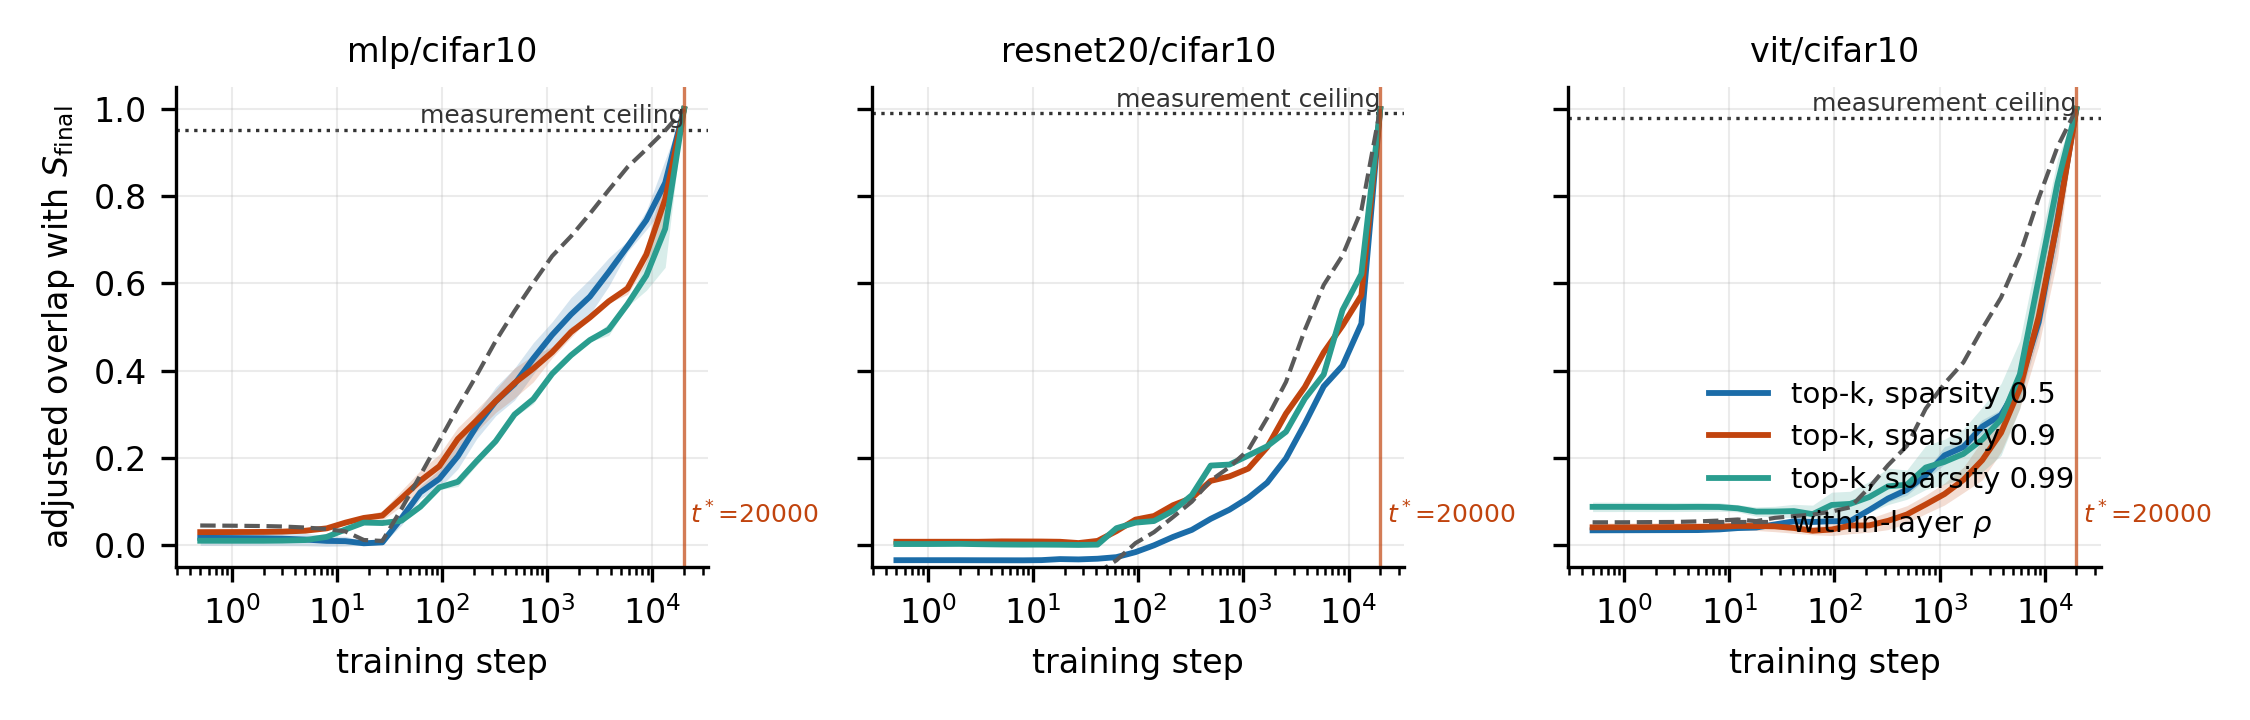
\includegraphics[width=\linewidth]{figures/fig1_stability.pdf}
  \caption{% TODO(final)
  Adjusted top-$k$ overlap with the final ordering. Dotted line: measurement ceiling from
  disjoint folds. Dashed: within-layer Spearman. Shaded: $\pm1$ s.d.\ over seeds.}
  \label{fig:stability}
\end{figure}
%% TODO(final): report t* per setting; state the three controls explicitly:
%%   (a) plateau sits below the fold ceiling  -> not estimator noise
%%   (b) adjusted overlap far above 0         -> not the layer budget
%%   (c) step-0 value below the plateau       -> not fixed at initialisation
%% and the budget/placement decomposition: which of the two settles first.

\begin{figure}[t]\centering
  \includegraphics[width=\linewidth]{figures/fig2_tstar.pdf}
  \caption{$t^*$ against width, depth, learning rate and batch size, and against kernel
  velocity. % TODO(final)
  }
  \label{fig:tstar}
\end{figure}

\section{Why: Jacobian motion and a heavy-tailed spectrum}
\label{sec:theory}
Write $a_i(\theta):=\sqrt{S_i(\theta)}=\|\partial F_\theta/\partial\theta_i\|_{L^2(\mu)}$,
the $L^2$ norm of the $i$th column of the Jacobian feature operator, and for two parameter
vectors set
$\Delta_i:=\|\partial F_{\theta}/\partial\theta_i-\partial F_{\theta'}/\partial\theta_i\|_{L^2(\mu)}$
and $\Delta:=\max_i\Delta_i$. Let $A_k(\theta)$ be the top-$k$ set of $a(\theta)$ and
$q_k(\theta)$ its $k$th largest entry.

\begin{proposition}[Trajectory rank stability]
\label{prop:stability}
For every $i$, $|a_i(\theta)-a_i(\theta')|\le\Delta_i$, and if the empirical Jacobian is
$L$-Lipschitz near the trajectory then
$\sum_i\Delta_i^2=\frac1n\|G_\theta-G_{\theta'}\|_F^2\le L^2\|\theta-\theta'\|_2^2$.
Moreover
\begin{equation}
  \big|A_k(\theta')\setminus A_k(\theta)\big|
  \;\le\;
  N_{\theta'}(2\Delta):=\#\{i:\ |a_i(\theta')-q_k(\theta')|\le 2\Delta\},
  \qquad
  \text{overlap}\;\ge\;1-\frac{N_{\theta'}(2\Delta)}{k}.
\end{equation}
\end{proposition}

\begin{proof}
The first claim is the reverse triangle inequality in $L^2(\mu;\mathbb R^{d_y})$; the
second is the definition of $\|G\|_F$ together with the Lipschitz assumption, applied
along the trajectory rather than across a pruning perturbation. For the third, the $k$th
order statistic is $1$-Lipschitz under a sup-norm perturbation, so
$|q_k(\theta)-q_k(\theta')|\le\Delta$. If $i\in A_k(\theta')\setminus A_k(\theta)$ then
$a_i(\theta')\ge q_k(\theta')$ and $a_i(\theta)<q_k(\theta)$, whence
$a_i(\theta')\le a_i(\theta)+\Delta< q_k(\theta)+\Delta\le q_k(\theta')+2\Delta$;
thus $0\le a_i(\theta')-q_k(\theta')<2\Delta$ and $i$ is counted by $N_{\theta'}(2\Delta)$.
\end{proof}

\begin{corollary}[Lazy conservation]
If $F$ is linear in $\theta$ along the trajectory, $G$ is constant, so $\Delta_i=0$ for all
$i$ and $A_k(\theta_t)=A_k(\theta_T)$ for every $t$ and $k$: the ordering is exactly
conserved. Observed rank churn is therefore a lower bound on departure from the linearised
regime.
\end{corollary}

\begin{corollary}[Heavy tails protect the boundary]
If the amplitude spectrum has density at most $\rho_k$ near $q_k$, then
$\text{overlap}\ge 1-2\Delta\rho_k p/k$. A heavy-tailed spectrum has low density at large
$k$, so the bound is non-vacuous precisely at the high sparsities where pruning operates,
and degrades in the dense bulk.
\end{corollary}

\begin{figure}[t]\centering
  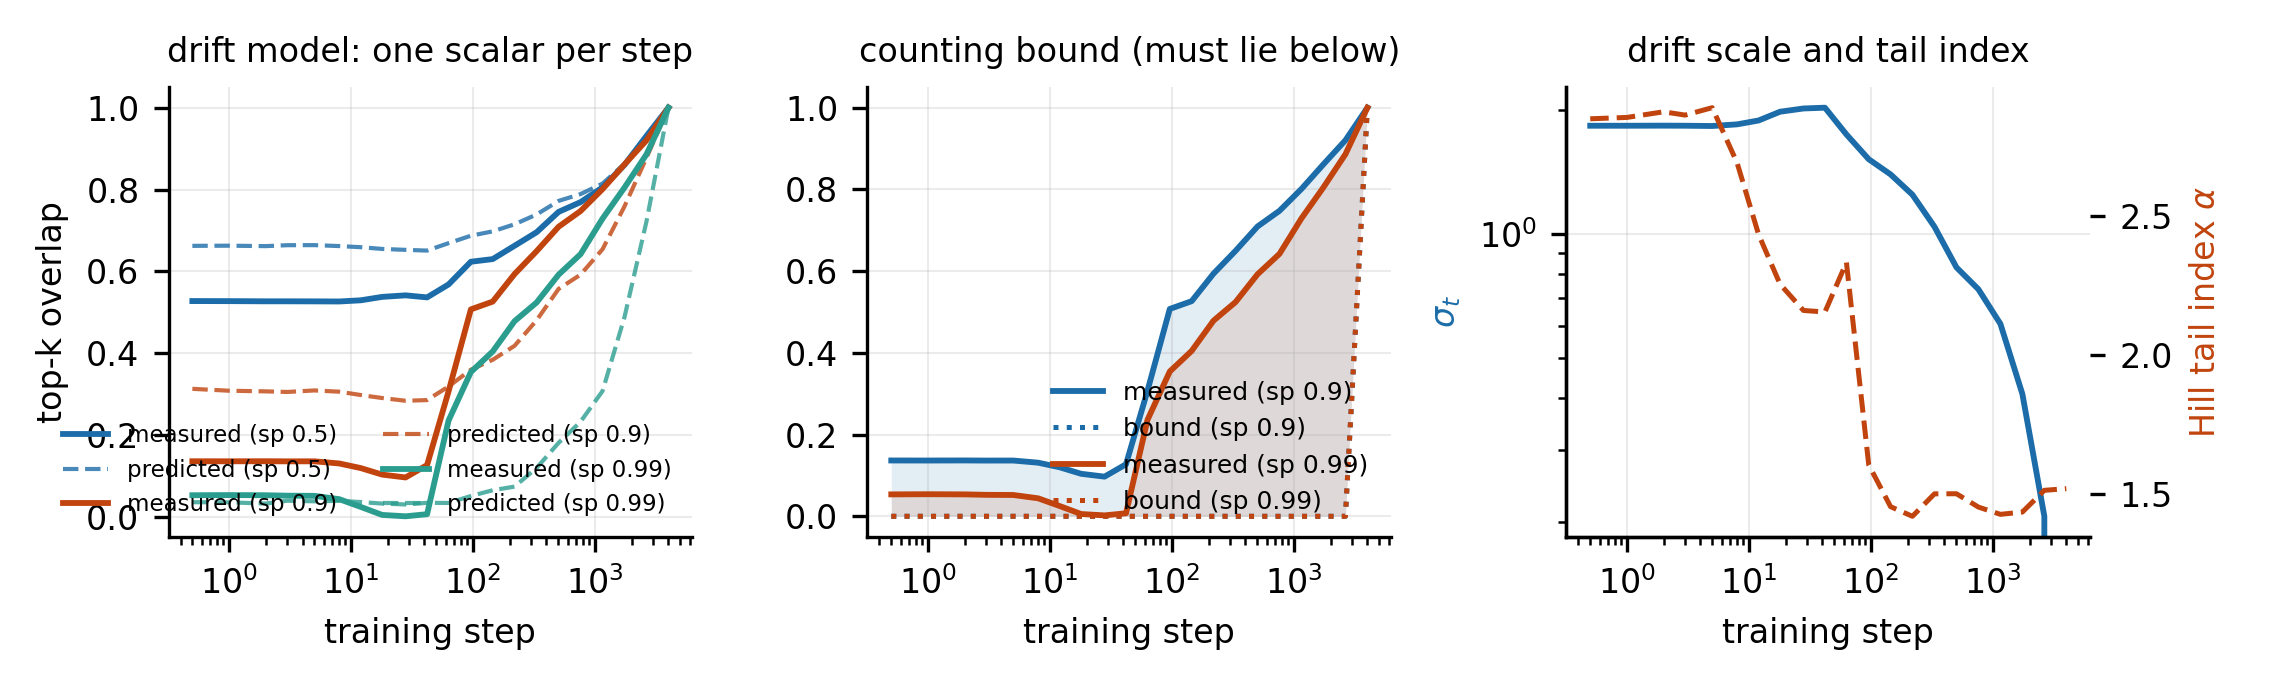
\includegraphics[width=\linewidth]{figures/fig3_theory.pdf}
  \caption{Left: the drift model predicts overlap at every sparsity from one measured
  scalar per checkpoint, with nothing fitted to the overlap curve. Centre: the bound of
  Prop.~\ref{prop:stability}. Right: drift scale and Hill tail index. % TODO(final)
  }
  \label{fig:theory}
\end{figure}
%% TODO(final): report (i) drift-model MAE, (ii) zero bound violations, (iii) the E4 result
%% -- t* collapsing as the laziness parameter alpha grows, which is the causal test.

\section{Consequence, limitations, and what comes next}
%% TODO(final): Fig 4 (accuracy vs prune time, t* marked). Keep this SHORT -- the pruning
%% study is the follow-up paper; here it establishes only that t* predicts the usable
%% prune time.
%% Limitations to state plainly: small models; single dataset family per architecture;
%% t* measured against S_final of the same run, so it is a statement about a trajectory,
%% not about transfer across runs; unstructured masks only.

\bibliographystyle{plainnat}
\bibliography{refs}
\end{document}
